\documentclass{article}  

% Chinese.
\usepackage[UTF8]{ctex}

% Page Layout.
\usepackage[left=.5in,right=.5in,top=.5in,bottom=.5in]{geometry}
\geometry{hmargin=0.4in,columnsep=0.3in,a4paper}

% Tables and graphics.
\usepackage{tabularx}
\usepackage{graphicx}

% Borders and header.
\usepackage{color}
\definecolor{myred}{rgb}{1.00, 0.545, 0.00}   % 西湖橙
\definecolor{myblue}{rgb}{0.00, 0.294, 0.686} % 西湖蓝色

% Hyperlinks.
\usepackage{hyperref}
\hypersetup{colorlinks=true,urlcolor=myblue}

% Justify lines.
\usepackage{ragged2e}

% Space between item in \enumerate.
\usepackage{enumitem}
\setlist{itemsep=0pt, parsep=4pt} % or \setlist{noitemsep} to leave space around whole list

\usepackage{soul} % for \ul: line-breaks version of \underline{}

% Set font style and size.
\usepackage[fontsize=10pt]{fontsize}
% \renewcommand{\familydefault}{\sfdefault}
\renewcommand{\baselinestretch}{1.2}

% Section and subsection styles.
\usepackage[explicit]{titlesec}
\titleformat{\section}{\large\bf\color{myred}}{\thesection}{1em}{\raggedright#1}
\titleformat{\subsection}{\normalsize\bf}{\thesubsection}{\normalsize}{\raggedright#1}
\titlespacing*{\section}{0pt}{0in}{-.2in}
\titlespacing*{\subsection}{0pt}{-.1in}{-.15in}

% Remove page number.
\pagenumbering{gobble}

% Space between paragraphs.
\setlength{\parskip}{\baselineskip}%
\setlength{\parindent}{0pt}

\begin{document}
% ---------------------- Author Address ---------------------- %
{\centering\bf\color{myred}
\LARGE ``分子模拟的理论与算法''课程作业平台\\\vskip.2em
\large ``Molecular Simulation: Theory and Algorithms'' Coursework Platform\\\vskip.5em
\LARGE 使用指南\\\vskip.2em
\large User Guide\\\vskip0.5em
}

\section*{平台登录 Accessing the Platform}

\begin{tabularx}{\linewidth}{l|X}
登录网址 URL & \url{https://hpc.westlake.edu.cn:7003/class-resource} \\
用户账号 Account  & 西湖大学学/工号\ \ \ \ \ \ \ Westlake University Identity and Access Management Platform UID \\
用户密码 Password & 西湖大学学/工号密码 Westlake University Identity and Access Management Platform Password
\end{tabularx}\vskip0.5em

\centerline{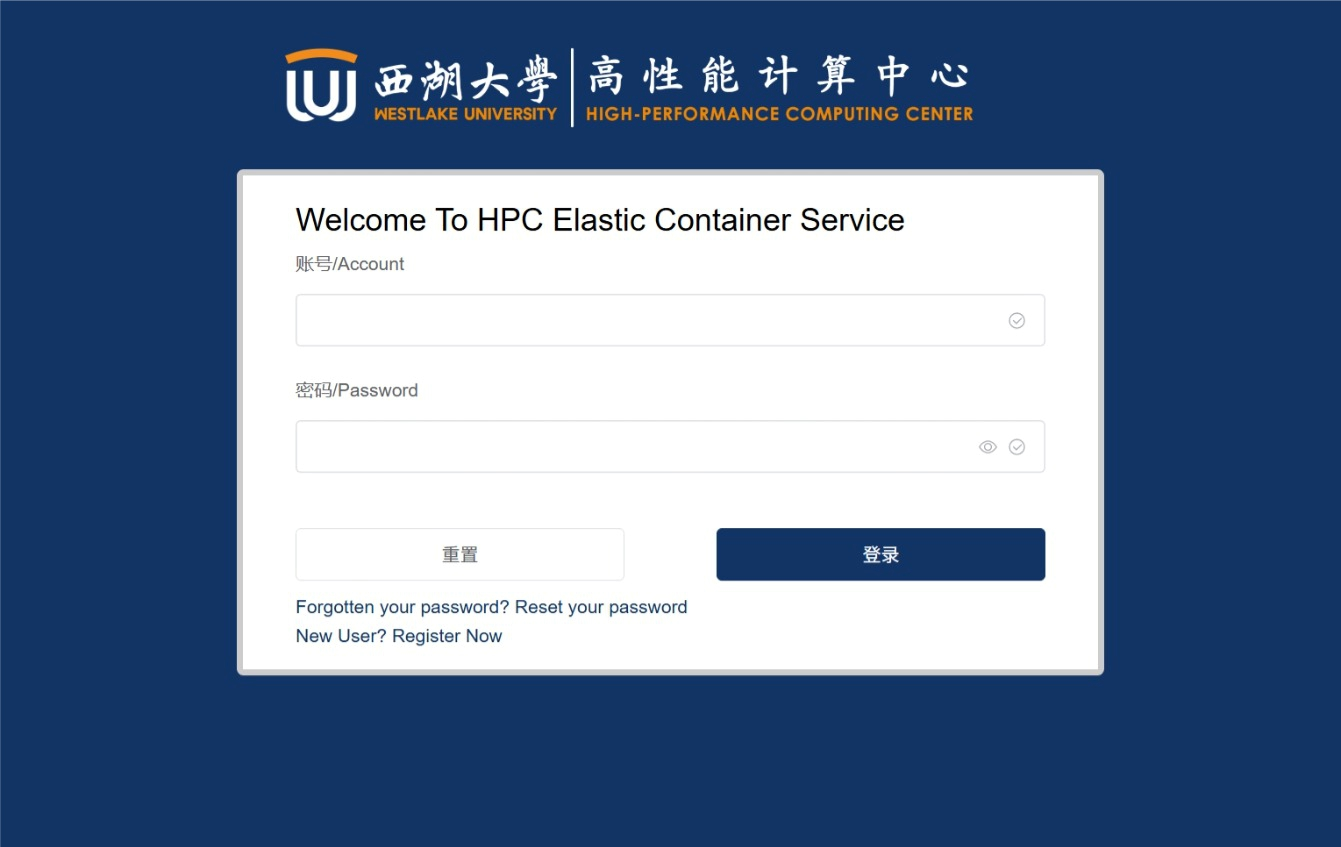
\includegraphics[scale=0.8]{figs/login0.jpg}}

登入平台后 when logged in,\\
1.点击``分子模拟的理论与算法''课程,click on ``分子模拟的理论与算法'';\\
2.点击``打开环境'' click on ``打开环境'';
\vskip0.5em

\centerline{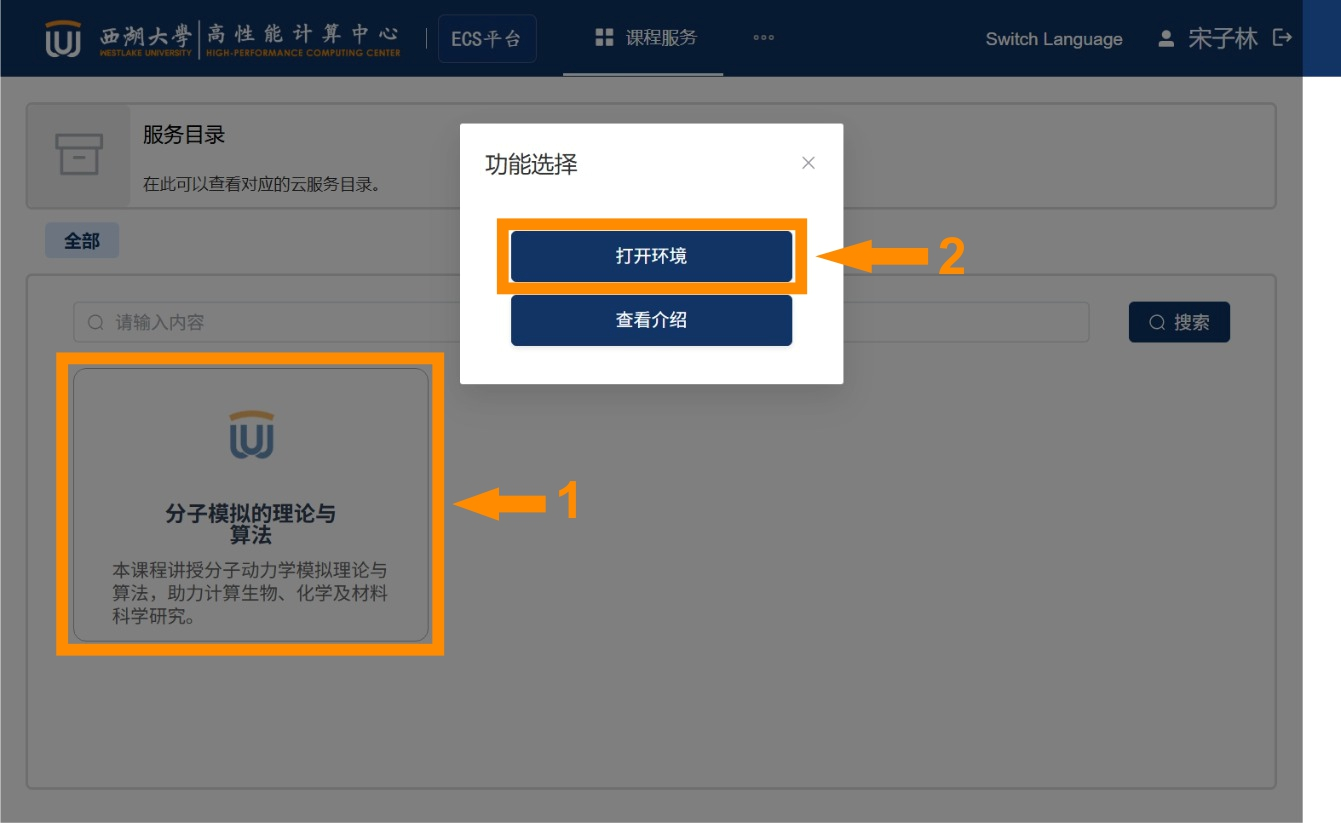
\includegraphics[scale=0.8]{figs/login1.jpg}}

3. 记录端口密码 copy the password;\\
4. 点击``网页访问'' click on ``网页访问''。
\vskip0.5em

\centerline{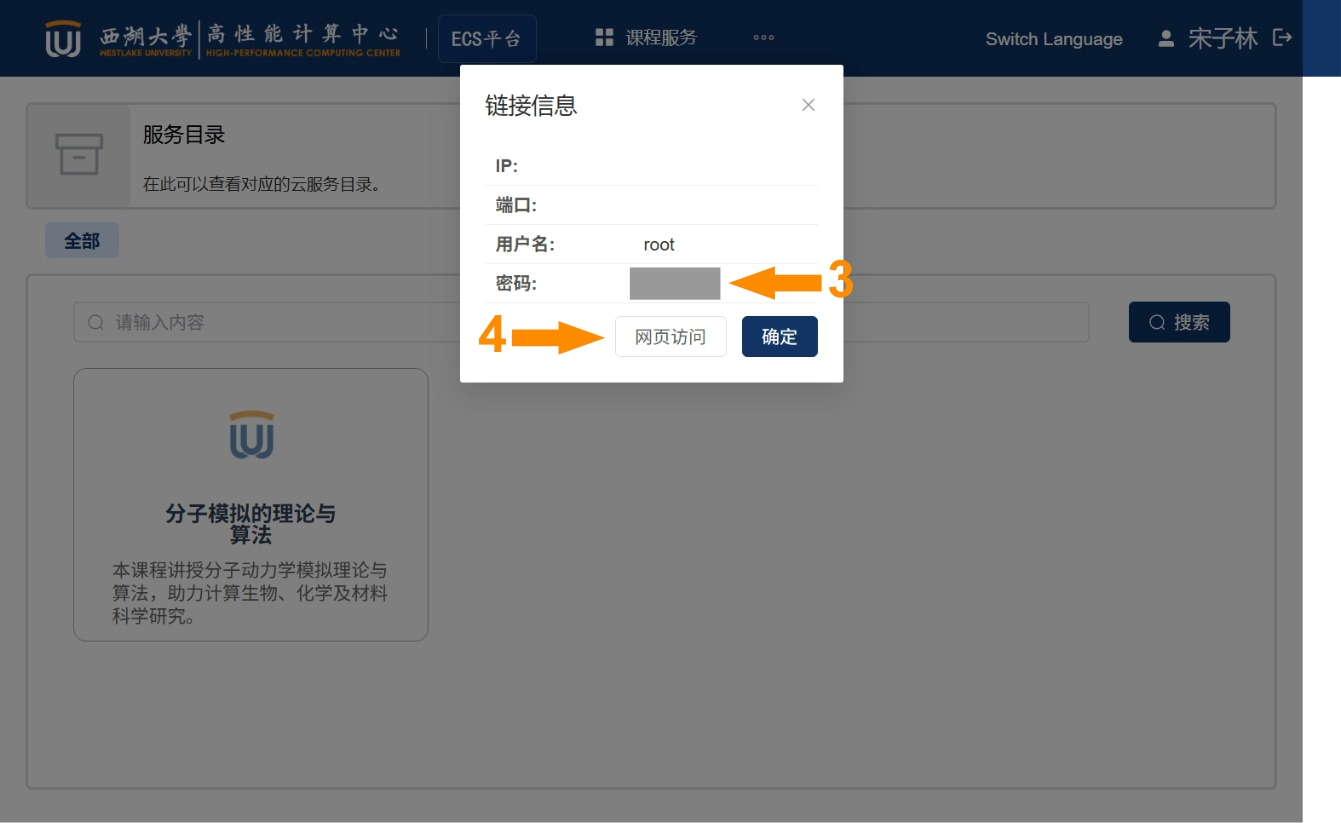
\includegraphics[scale=0.8]{figs/login2.jpg}}

5. 输入端口密码并进入作业环境 enter the password and login the coursework environment。
\vskip0.5em

\centerline{
\includegraphics[scale=0.8]{figs/login3.jpg}}

如果用户登录遇到问题,请联系课程助教。\\
Consult your teaching assistant for login issues.

\section*{平台简介 Introducing the Platform}

课程作业主要依托 JupyterLab 平台。界面左侧为文件管理器(橙色),右侧为工作区(蓝色)。\\
The left part (orange region) is the File Explorer and the right part (blue region) is the workspace。
\vskip0.5em

\centerline{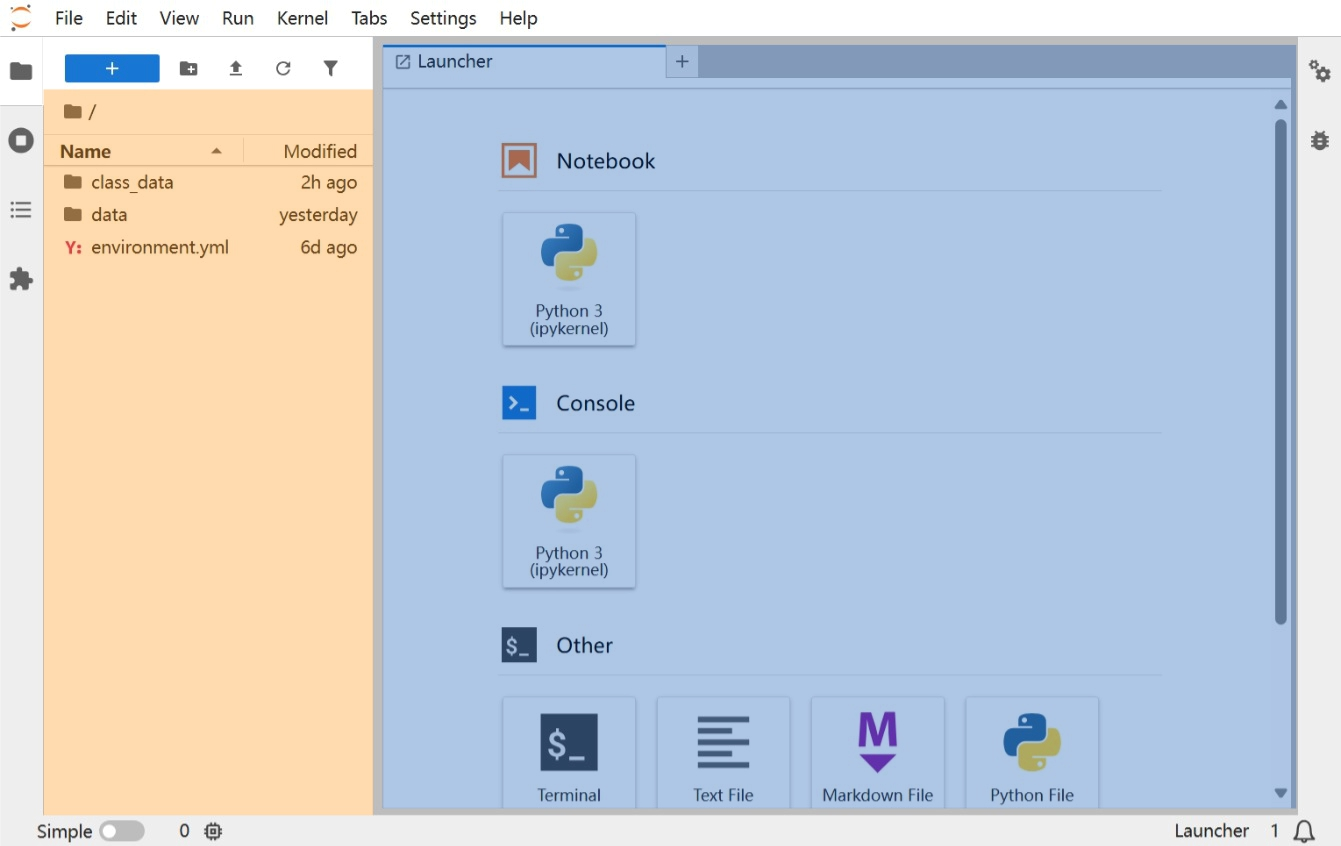
\includegraphics[scale=0.8]{figs/system0.jpg}}

在文件管理器中
\begin{itemize}
  \item `class\_data' 文件夹包含一些课程资料以及作业模板,学员仅拥有只读权限(学员不可直接编辑该文件夹中的文件/编辑后无法保存);
    \begin{itemize}
      \item `class\_data/assignments' 文件夹包含每次课程作业的模板文件,学员可在 `data' 文件夹下复制每次作业的对应模板进行编辑;
      \item `class\_data/mdpy' 文件夹包含\textsc{MDPy}程序的源代码,是基于Python实现的分子动力学模拟基础代码模块。学员可在 `data' 文件夹下复制该文件夹进行编辑;
      \item `class\_data/md\_demo.ipynb' 文件是利用\textsc{MDPy}模块实现一个简单分子动力学模拟的JupyterLab示例(JupyterLab使用说明见~\hyperref[sec:ref]{参考资料 References}),学员可自主运行各代码模块以查看模拟结果和计算细节。
    \end{itemize}
  \item `data' 文件夹为学员的作业区,学员拥有读写权限。
\end{itemize}

此外,其他文件路径下的文件或数据均非持久化存储。\\
{\bf
\color{myred} 在退出平台或关闭端口之后,除了位于 `data' 和 `class\_data' 下的其他数据或文件将在再次登陆时丢失。\\
\color{myblue}在退出平台或关闭端口之后,除了位于 `data' 和 `class\_data' 下的其他数据或文件将在再次登陆时丢失。\\
\color{myred} 在退出平台或关闭端口之后,除了位于 `data' 和 `class\_data' 下的其他数据或文件将在再次登陆时丢失。}

{\bf 学员应全程都在 `data' 文件夹下完成和测试作业代码。}

以安全合理的方式保存研究数据是科学研究的基本技能,我们不对学员因非持久化储存所导致的数据丢失负责。

\section*{作业准备 Preparing for the assignments}

所有课程作业的内容围绕分子动力学模拟的算法实现开展。
平台提供了用于简单模型体系分子动力学模拟的\textsc{MDPy}程序,尽管学员无需了解其实现细节,在每次作业中,学员将在给出的作业样例的指导下利用\textsc{MDPy}的预设接口实现并测试分子动力学模拟算法。

以第一次作业为例,学员应当进行如下准备工作:\\
1. 将 `class\_data/mdpy' 文件夹整体复制到 `data' 文件夹下;\\
2. 将 `class\_data/assignments' 文件夹下的当次作业的 `1\_integrators.ipynb' 文件复制到 `data' 文件夹下;\\
3. 根据 `data/1\_integrators.ipynb' 中的指示,在其中完成第一次作业。其中\textbf{1}-\textbf{3}为作业内容介绍及\textsc{MDPy}程序说明,\textbf{4}为作业示例。学员应在\textbf{5. Your Answer}部分根据作业要求完成作业,具体包括\textbf{5.1} 预备实现的积分器及其公式推导(Markdown语法)、\textbf{5.2} Python 代码实现及\textbf{5.3} 积分器使用测试。学员应在代码中提供清晰的注释以说明实现细节。\\

\centerline{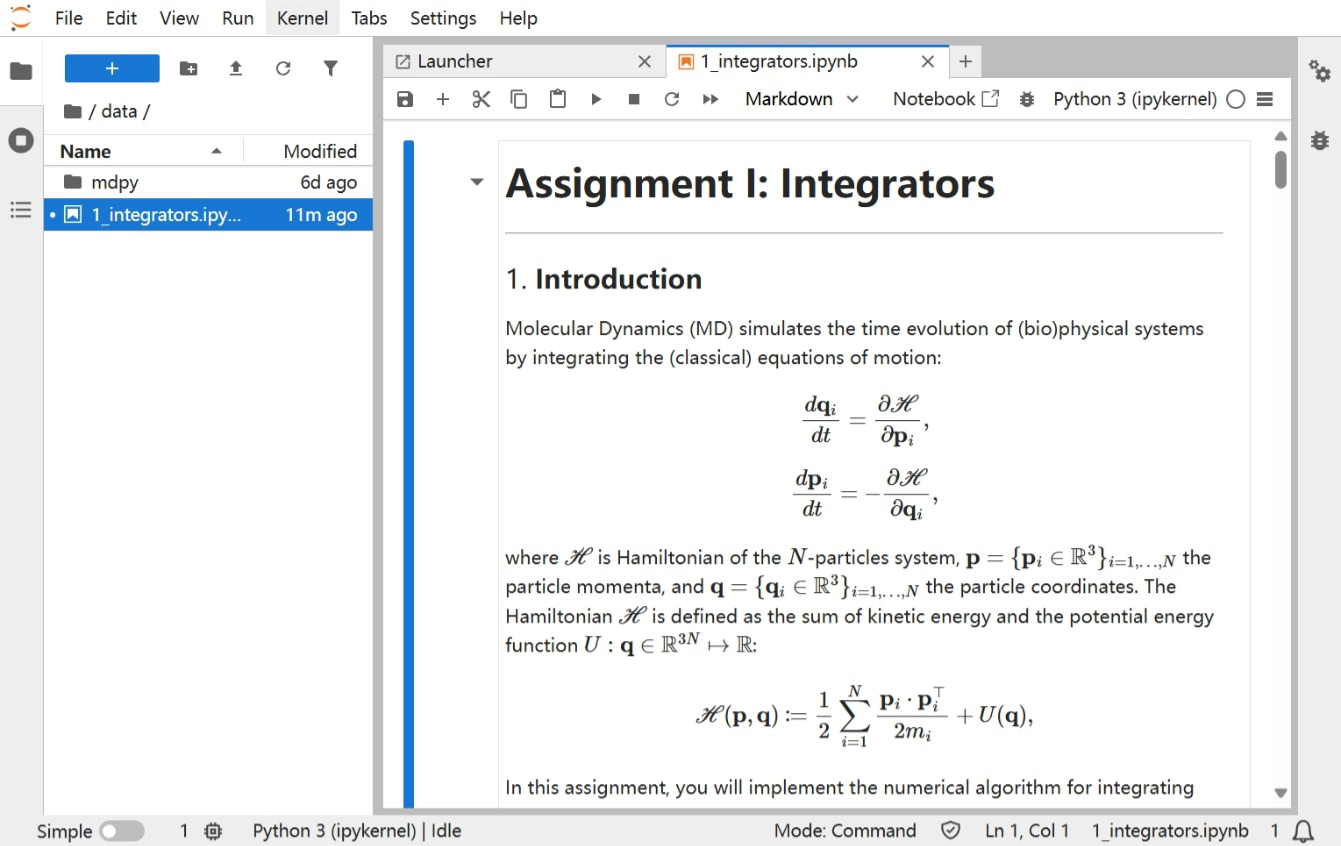
\includegraphics[scale=0.8]{figs/system1.jpg}}

\section*{作业提交 Submitting for the assignments}

学员完成作业后,将作业文件(例如`1\_integrators.ipynb')保存在`data'中即可,主讲教师能够查看学员账户中的`data'文件夹下的全部内容。

\section*{注意事项 Important notes}

\begin{enumerate}
  \item 如果学员保存了同一次作业的多个副本,\textbf{主讲教师将仅查看编辑时间最晚的作业副本}。
  \item 如果学员在当次作业的截止时间后修改了作业文件,则需要通知主讲教师,\textbf{否则我们将仅查看截止时间前的作业文件}。
  \item 如果学员的实现涉及对\textsc{MDPy}源代码的修改,\textbf{则需要给出详细的修改位置及原因,否则将被视为实现错误}。
  \item 如果学员在完成作业的过程中受益于他人的指导或讨论,\textbf{则需要在作业中明确致谢},这将不会对作业评价产生负面影响。
  \item \textbf{禁止共享账号或代替他人完成作业 Account sharing or proxy submissions are strictly prohibited}。
  \item {\bf \color{myred} 截止时间前请务必确认所有待提交作业内容已置于`data'目录下!!!}
\end{enumerate}

\section*{参考资料 References}
\phantomsection\label{sec:ref}
\begin{itemize}
  \item \href{https://jupyterlab.readthedocs.io/en/latest/user/}{JupyterLab使用指南}
  \item \href{https://medium.com/@tuenguyends/start-your-first-project-with-jupyter-lab-84f5b78b4522#:~:text=Create%20your%20first%20notebook}{JupyterLab使用示例}
  \item \href{https://markdown.com.cn/}{Markdown教程},或在Jupyter Notebook界面中点击`Help'下拉菜单中的`Markdown Reference'
  \item \href{https://simpletex.cn/ai/latex_ocr}{SimpleTex},可帮助将图片或照片中的公式转换为Markdown语法。
  \item \href{https://liaoxuefeng.com/books/python/basic/index.html}{Python基础教程}
\end{itemize}

\end{document}